%&../../.preamble
\externalize{../../.preamble}

\usepackage{contour}

\title{Ripetizioni Matteo}
\author{Marini Mattia}
\date{2024}

\begin{document}
\maketitle
\license{Ripetizioni Matteo}
\tableofcontents
\listofdefs
% \listoftheorems
% \listofexercises

\newpage
\section{Equazioni di secondo grado}
\subsection{Terminologia}
\begin{definizione}{Forma normale}
	Un'equazione si dice in forma normale se è scritta come un'equzione tra un polinomio e zero e non si può semplificare nulla
\end{definizione}
\begin{itemize}
	\item Equazioni in forma normale:
	      \begin{align*}
		      15x^{4} + x^2  -2x + 2 = 0 &  & 12x = 0 &  & x^2 + 1 = 0
	      \end{align*}
	\item Equazioni che \underline{NON} sono in forma normale:
	      \begin{align*}
		       & 12x = 1 &  & x^2 - x^2  +x = 0
	      \end{align*}
\end{itemize}
non lo sono.

\begin{definizione}{Equazione di secondo grado}
	Un'equazione si dice di secondo grado se, una volta ridotta in forma normale l'esponente di grado massimo è uguale a 2
\end{definizione}
\begin{itemize}
	\item Equazioni di secondo grado:
	      \begin{align*}
		       & 5x^2 -2x + 1 = 0 &  & 5x^2 -2x + 1 = 2x^2  -2 \\
		       & x^2  = -1        &  & x^2 -2x = 0
	      \end{align*}
	\item Equazioni che \underline{NON} sono di secondo grado:
	      \begin{align*}
		       & 2x + 1 = 0     &  & 5x^2 -5x^2  + 1 =  -2 \\
		       & x^2  = x^2 + x &  & 3x + 2 = -2x
	      \end{align*}
\end{itemize}

\begin{definizione}{Equazioni complete, pure, spurie, monomie}
	Un' equazione di \underline{secondo grado} può essere classificata in base a quali suoi coefficienti valgono. Una generica equazione di secondo grado
	\[
		ax^2  + bx + c = 0
	\]
	viene detta:
	\begin{itemize}
		\item \textit{Completa} se ne $ a $ ne $ b $ ne $ c $ valgono 0: $ 15x^2  + 2x -10 = 0  $
		\item \textit{Pura} se solo $ b = 0 $: $ 15x^2  - 10 = 0 $
		\item \textit{Spuria} se solo $ c = 0 $: $ 15x^2 +2x = 0  $
		\item \textit{Monomia} se sia $ b $ che $ c $ valgono 0: $ 15x^2 = 0 $
	\end{itemize}
\end{definizione}\label{tipiequazionisecondogrado}

\subsection{Risoluzione equazioni di secondo grado}
Ci occupiamo intanto della risoluzione delle equazioni \underline{NON} fratte. Lo schema risolutivo è il seguente:
\begin{enumerate}
	\item Tramite le proprietà delle equazioni, riduco al l'equazione nella sua \underline{forma normale}
	\item Trovare i risultati come indicato qui sotto, in base al tipo della equazione ottenuta vedi definizione \ref{tipiequazionisecondogrado}
\end{enumerate}
\subsubsection{Equazioni complete}
Per questo tipo di equazione esiste una formula nella quale possiamo inserire i parametri per ricavare le soluzioni. Data un'equazione di secondo grado nella seguente forma:
\[
	ax^2  + bx + c = 0
\]
allora le soluzioni sono date da
\[
	x_{1/2} = \frac{-b \pm \sqrt{b^2  - 4 ac}}{2a}
\]
nota che
\begin{itemize}
	\item La quantità $ \sqrt{b^2  - 4ac} $ è detta \underline{determinante} e si indica con $ \Delta  $
	\item Questa formula può produrre 0,1 o 2 soluzioni a seconda del valore di $ \Delta  $:
	      \begin{itemize}
		      \item $ \Delta < 0 $: 0 soluzioni
		      \item $ \Delta = 0 $: 1 soluzione
		      \item $ \Delta > 0 $: 2 soluzioni
	      \end{itemize}
\end{itemize}
\subsubsection*{Esempio}
Supponendo di avere:
\[
	2x^2  - 4x - 6
\]
le soluzioni sono date da
\begin{center}
	\begin{tikzpicture}
		\node (formula)[] at (0,0) {$ \displaystyle x_{1/2} = \frac{4 \pm \sqrt{\left(-4\right)^2  - 4 (2) \cdot (-6)}}{2 \cdot 2} = \frac{4 \pm \sqrt{64}}{4} = \frac{4 \pm 8}{4}$};
		\node (solution1)[above right = -0.5em and 2em of formula] {$ \displaystyle x_1 = \frac{12}{4} = 3 $};
		\node (solution2)[below right = -0.5em and 2em of formula]  {$ \displaystyle x_2 = \frac{-4}{4} = -1 $};
		\draw [->] (formula.east) to [out=0, in=180] (solution1.west);
		\draw [->] (formula.east) to [out=0, in=180] (solution2.west);
	\end{tikzpicture}
\end{center}

\subsubsection{Equazioni pure}
Per questo tipo di equazioni è sufficiente portare a destra $ a $ e $ c $ ed eseguire la radice da entrambe le parti. Occhio al "$ \pm $"!
\[
	ax^2 + c  = 0 \rightarrow ax^2  = -c \rightarrow x^2  = \frac{-c}{a} \rightarrow x = \pm \sqrt{\frac{-c}{a}}
\]
Nota che
\begin{itemize}
	\item Nell'ultimo passaggio va messo sempre il $ \pm $. Basti pensare a $ x^2  = 4 $. Chiaramente $ 2 \cdot 2 = 4 $ ma anche $ -2 \cdot  -2  = 4$. Questo è vero per \underline{qualsiasi numbero}!
	\item Le equazioni pure hanno sempre 2 o 0 soluzioni, nel caso alla destra io ottenga rispettivamente un numero positivo o negativo
\end{itemize}
\subsubsection*{Esempio}
Supponendo di avere:
\[
	4x^2 -9 = 0
\]
allora procedo così:
\[
	4x^2 = 9 \rightarrow \sqrt{4x^2 } = \sqrt{9} \rightarrow 2x = 3 \rightarrow x = \frac{3}{2}
\]

\subsubsection{Equazioni spurie}
Per questo tipo di equazioni si può sempre effettuare un raccoglimento della $ x $, applicando poi la legge dell'annullamento del prodotto:
\begin{center}
	\begin{tikzpicture}
		\node (formula)[] at (0,0) {$ \displaystyle ax^2  + bx = 0 \rightarrow x\left(ax + b\right) = 0 $};
		\node (solution1)[above right = -0.5em and 2em of formula] {$ \displaystyle x_1 = 0 $};
		\node (solution2)[below right = -0.5em and 2em of formula]  {$ \displaystyle x_2 = \frac{-b}{a} $};
		\draw [->] (formula.east) to [out=0, in=180] (solution1.west);
		\draw [->] (formula.east) to [out=0, in=180] (solution2.west);
	\end{tikzpicture}
\end{center}

Nota che:
\begin{itemize}
	\item Ho sempre esattamente 2 soluzioni
	\item Una soluzione è sempre 0. Questo perché la $ x $ compare in ogni fattore. Quando questa si annulla, l'equazione sarà sempre soddisfatta
\end{itemize}

\subsubsection*{Esempio}
Supponiamo di avere:
\[
	5x^2  - 2x = 0
\]
allora risolvo così
\begin{center}
	\begin{tikzpicture}
		\node (formula)[] at (0,0) {$ \displaystyle 5x^2 -2x = 0 \rightarrow x\left(5x - 2\right) = 0 $};
		\node (solution1)[above right = -0.5em and 2em of formula] {$ \displaystyle x_1 = 0 $};
		\node (solution2)[below right = -0.5em and 2em of formula]  {$ \displaystyle \left(5x-2\right) = 0 \rightarrow x_2 = \frac{5}{2} $};
		\draw [->] (formula.east) to [out=0, in=180] (solution1.west);
		\draw [->] (formula.east) to [out=0, in=180] (solution2.west);
	\end{tikzpicture}
\end{center}

\subsubsection{Monomie}
Il caso delle equazioni monomie è particolarmente semplice. La soluzione è \underline{una}, ossia 0
\[
	ax^2 = 0 \rightarrow x = 0
\]

\subsection{Esercizi}

\subsubsection{Pure}
\begin{align*}
	 & 5x^2 - 20 = 0 &  & 3x^2 - 27 = 0 &  & 4x^2 - 36 = 0 \\
	 & 2x^2 - 8 = 0  &  & x^2 - 16 = 0  &  & 6x^2 - 18 = 0 \\
\end{align*}

\textit{Soluzione 1}\vskip3mm
\[
	5x^2 - 20 = 0 \rightarrow 5x^2 = 20 \rightarrow x^2 = 4 \rightarrow x = \pm 2
\]

\textit{Soluzione 2}\vskip3mm
\[
	3x^2 - 27 = 0 \rightarrow 3x^2 = 27 \rightarrow x^2 = 9 \rightarrow x = \pm 3
\]

\textit{Soluzione 3}\vskip3mm
\[
	4x^2 - 36 = 0 \rightarrow 4x^2 = 36 \rightarrow x^2 = 9 \rightarrow x = \pm 3
\]

\textit{Soluzione 4}\vskip3mm
\[
	2x^2 - 8 = 0 \rightarrow 2x^2 = 8 \rightarrow x^2 = 4 \rightarrow x = \pm 2
\]

\textit{Soluzione 5}\vskip3mm
\[
	x^2 - 16 = 0 \rightarrow x^2 = 16 \rightarrow x = \pm 4
\]

\textit{Soluzione 6}\vskip3mm
\[
	6x^2 - 18 = 0 \rightarrow 6x^2 = 18 \rightarrow x^2 = 3 \rightarrow x = \pm \sqrt{3}
\]

\subsubsection{Spurie}
\begin{align*}
	 & 4x^2 - 8x = 0 &  & 6x^2 - 18x = 0 &  & 5x^2 - 10x = 0 \\
	 & 3x^2 - 9x = 0 &  & 2x^2 - 4x = 0  &  & 7x^2 - 21x = 0 \\
\end{align*}


\textit{Soluzione 1}
\vskip3mm

\begin{center}
	\begin{tikzpicture}
		\node (formula)[] at (0,0) {$ \displaystyle 4x^2 - 8x = 0 \rightarrow x\left(4x - 8\right) = 0 $};
		\node (solution1)[above right = -0.5em and 2em of formula] {$ \displaystyle x_1 = 0 $};
		\node (solution2)[below right = -0.5em and 2em of formula] {$ \displaystyle x_2 = 2 $};
		\draw [->] (formula.east) to [out=0, in=180] (solution1.west);
		\draw [->] (formula.east) to [out=0, in=180] (solution2.west);
	\end{tikzpicture}
\end{center}

\textit{Soluzione 2}
\vskip3mm
\begin{center}
	\begin{tikzpicture}
		\node (formula)[] at (0,0) {$ \displaystyle 6x^2 - 18x = 0 \rightarrow x\left(6x - 18\right) = 0 $};
		\node (solution1)[above right = -0.5em and 2em of formula] {$ \displaystyle x_1 = 0 $};
		\node (solution2)[below right = -0.5em and 2em of formula] {$ \displaystyle x_2 = 3 $};
		\draw [->] (formula.east) to [out=0, in=180] (solution1.west);
		\draw [->] (formula.east) to [out=0, in=180] (solution2.west);
	\end{tikzpicture}
\end{center}

\textit{Soluzione 3}
\vskip3mm
\begin{center}
	\begin{tikzpicture}
		\node (formula)[] at (0,0) {$ \displaystyle 5x^2 - 10x = 0 \rightarrow x\left(5x - 10\right) = 0 $};
		\node (solution1)[above right = -0.5em and 2em of formula] {$ \displaystyle x_1 = 0 $};
		\node (solution2)[below right = -0.5em and 2em of formula] {$ \displaystyle x_2 = 2 $};
		\draw [->] (formula.east) to [out=0, in=180] (solution1.west);
		\draw [->] (formula.east) to [out=0, in=180] (solution2.west);
	\end{tikzpicture}
\end{center}

\textit{Soluzione 4}
\vskip3mm
\begin{center}
	\begin{tikzpicture}
		\node (formula)[] at (0,0) {$ \displaystyle 3x^2 - 9x = 0 \rightarrow x\left(3x - 9\right) = 0 $};
		\node (solution1)[above right = -0.5em and 2em of formula] {$ \displaystyle x_1 = 0 $};
		\node (solution2)[below right = -0.5em and 2em of formula] {$ \displaystyle x_2 = 3 $};
		\draw [->] (formula.east) to [out=0, in=180] (solution1.west);
		\draw [->] (formula.east) to [out=0, in=180] (solution2.west);
	\end{tikzpicture}
\end{center}

\textit{Soluzione 5}
\vskip3mm
\begin{center}
	\begin{tikzpicture}
		\node (formula)[] at (0,0) {$ \displaystyle 2x^2 - 4x = 0 \rightarrow x\left(2x - 4\right) = 0 $};
		\node (solution1)[above right = -0.5em and 2em of formula] {$ \displaystyle x_1 = 0 $};
		\node (solution2)[below right = -0.5em and 2em of formula] {$ \displaystyle x_2 = 2 $};
		\draw [->] (formula.east) to [out=0, in=180] (solution1.west);
		\draw [->] (formula.east) to [out=0, in=180] (solution2.west);
	\end{tikzpicture}
\end{center}

\textit{Soluzione 6}
\vskip3mm
\begin{center}
	\begin{tikzpicture}
		\node (formula)[] at (0,0) {$ \displaystyle 7x^2 - 21x = 0 \rightarrow x\left(7x - 21\right) = 0 $};
		\node (solution1)[above right = -0.5em and 2em of formula] {$ \displaystyle x_1 = 0 $};
		\node (solution2)[below right = -0.5em and 2em of formula] {$ \displaystyle x_2 = 3 $};
		\draw [->] (formula.east) to [out=0, in=180] (solution1.west);
		\draw [->] (formula.east) to [out=0, in=180] (solution2.west);
	\end{tikzpicture}
\end{center}


\subsubsection{Complete}
\begin{align*}
	 & 3x^2 - 4x - 7 = 0 &  & 5x^2 + 8x - 3 = 0  &  & 2x^2 - 6x + 4 = 0  \\
	 & x^2 - 2x - 8 = 0  &  & 4x^2 + 12x + 5 = 0 &  & 6x^2 - 11x + 2 = 0 \\
\end{align*}

\textit{Soluzione 1:}
\begin{align*}
	 & 3x^2 - 4x - 7 = 0 &  & \underbracket[0.1ex]{(3)}_{a}x^2 + \underbracket[0.1ex]{(-4)}_{b}x + \underbracket[0.1ex]{(-7)}_{c} = 0
\end{align*}
\begin{center}
	\begin{tikzpicture}
		\node (formula)[] at (0,0) {$ \displaystyle x_{1/2} = \frac{-(-4) \pm \sqrt{(-4)^2 - 4 \cdot 3 \cdot (-7)}}{2 \cdot 3}  = \frac{4 \pm \sqrt{100}}{6} $};
		\node (solution1)[above right = -0.5em and 2em of formula] {$ \displaystyle x_1 = \frac{4 + 10}{3} $};
		\node (solution2)[below right = -0.5em and 2em of formula]  {$ \displaystyle x_2 = \frac{4 - 10}{3} $};
		\draw [->] (formula.east) to [out=0, in=180] (solution1.west);
		\draw [->] (formula.east) to [out=0, in=180] (solution2.west);
	\end{tikzpicture}
\end{center}

\textit{Soluzione 1:}
\begin{align*}
	 & 3x^2 - 4x - 7 = 0 &  & \underbracket[0.1ex]{(3)}_{a}x^2 + \underbracket[0.1ex]{(-4)}_{b}x + \underbracket[0.1ex]{(-7)}_{c} = 0
\end{align*}
\begin{center}
	\begin{tikzpicture}
		\node (formula)[] at (0,0) {$ \displaystyle x_{1/2} = \frac{-(-4) \pm \sqrt{(-4)^2 - 4 \cdot 3 \cdot (-7)}}{2 \cdot 3}  = \frac{4 \pm \sqrt{100}}{6} $};
		\node (solution1)[above right = -0.5em and 2em of formula] {$ \displaystyle x_1 = \frac{2 + \sqrt{10}}{3} $};
		\node (solution2)[below right = -0.5em and 2em of formula]  {$ \displaystyle x_2 = \frac{2 - \sqrt{10}}{3} $};
		\draw [->] (formula.east) to [out=0, in=180] (solution1.west);
		\draw [->] (formula.east) to [out=0, in=180] (solution2.west);
	\end{tikzpicture}
\end{center}

\textit{Soluzione 2:}
\begin{align*}
	 & 5x^2 + 8x - 3 = 0 &  & \underbracket[0.1ex]{(5)}_{a}x^2 + \underbracket[0.1ex]{(8)}_{b}x + \underbracket[0.1ex]{(-3)}_{c} = 0
\end{align*}
\begin{center}
	\begin{tikzpicture}
		\node (formula)[] at (0,0) {$ \displaystyle x_{1/2} = \frac{-8 \pm \sqrt{8^2 - 4 \cdot 5 \cdot (-3)}}{2 \cdot 5}  = \frac{-8 \pm \sqrt{124}}{10} $};
		\node (solution1)[above right = -0.5em and 2em of formula] {$ \displaystyle x_1 = \frac{-4 + \sqrt{31}}{5} $};
		\node (solution2)[below right = -0.5em and 2em of formula]  {$ \displaystyle x_2 = \frac{-4 - \sqrt{31}}{5} $};
		\draw [->] (formula.east) to [out=0, in=180] (solution1.west);
		\draw [->] (formula.east) to [out=0, in=180] (solution2.west);
	\end{tikzpicture}
\end{center}

\textit{Soluzione 3:}
\begin{align*}
	 & 2x^2 - 6x + 4 = 0 &  & \underbracket[0.1ex]{(2)}_{a}x^2 + \underbracket[0.1ex]{(-6)}_{b}x + \underbracket[0.1ex]{(4)}_{c} = 0
\end{align*}
\begin{center}
	\begin{tikzpicture}
		\node (formula)[] at (0,0) {$ \displaystyle x_{1/2} = \frac{-(-6) \pm \sqrt{(-6)^2 - 4 \cdot 2 \cdot 4}}{2 \cdot 2}  = \frac{6 \pm \sqrt{4}}{4} $};
		\node (solution1)[above right = -0.5em and 2em of formula] {$ \displaystyle x_1 = \frac{4}{4} = 1 $};
		\node (solution2)[below right = -0.5em and 2em of formula]  {$ \displaystyle x_2 = \frac{2}{4} = \frac{1}{2} $};
		\draw [->] (formula.east) to [out=0, in=180] (solution1.west);
		\draw [->] (formula.east) to [out=0, in=180] (solution2.west);
	\end{tikzpicture}
\end{center}

\textit{Soluzione 4:}
\begin{align*}
	 & x^2 - 2x - 8 = 0 &  & \underbracket[0.1ex]{(1)}_{a}x^2 + \underbracket[0.1ex]{(-2)}_{b}x + \underbracket[0.1ex]{(-8)}_{c} = 0
\end{align*}
\begin{center}
	\begin{tikzpicture}
		\node (formula)[] at (0,0) {$ \displaystyle x_{1/2} = \frac{-(-2) \pm \sqrt{(-2)^2 - 4 \cdot 1 \cdot (-8)}}{2 \cdot 1}  = \frac{2 \pm \sqrt{36}}{2} $};
		\node (solution1)[above right = -0.5em and 2em of formula] {$ \displaystyle x_1 = \frac{2 + 6}{2} = 4 $};
		\node (solution2)[below right = -0.5em and 2em of formula]  {$ \displaystyle x_2 = \frac{2 - 6}{2} = -2 $};
		\draw [->] (formula.east) to [out=0, in=180] (solution1.west);
		\draw [->] (formula.east) to [out=0, in=180] (solution2.west);
	\end{tikzpicture}
\end{center}

\textit{Soluzione 5:}
\begin{align*}
	 & 4x^2 + 12x + 5 = 0 &  & \underbracket[0.1ex]{(4)}_{a}x^2 + \underbracket[0.1ex]{(12)}_{b}x + \underbracket[0.1ex]{(5)}_{c} = 0
\end{align*}
\begin{center}
	\begin{tikzpicture}
		\node (formula)[] at (0,0) {$ \displaystyle x_{1/2} = \frac{-12 \pm \sqrt{12^2 - 4 \cdot 4 \cdot 5}}{2 \cdot 4}  = \frac{-12 \pm \sqrt{64}}{8} $};
		\node (solution1)[above right = -0.5em and 2em of formula] {$ \displaystyle x_1 = \frac{-8}{8} = -1 $};
		\node (solution2)[below right = -0.5em and 2em of formula]  {$ \displaystyle x_2 = \frac{-2}{8} = -\frac{1}{4} $};
		\draw [->] (formula.east) to [out=0, in=180] (solution1.west);
		\draw [->] (formula.east) to [out=0, in=180] (solution2.west);
	\end{tikzpicture}
\end{center}

\textit{Soluzione 6:}
\begin{align*}
	 & 6x^2 - 11x + 2 = 0 &  & \underbracket[0.1ex]{(6)}_{a}x^2 + \underbracket[0.1ex]{(-11)}_{b}x + \underbracket[0.1ex]{(2)}_{c} = 0
\end{align*}
\begin{center}
	\begin{tikzpicture}
		\node (formula)[] at (0,0) {$ \displaystyle x_{1/2} = \frac{-(-11) \pm \sqrt{(-11)^2 - 4 \cdot 6 \cdot 2}}{2 \cdot 6}  = \frac{11 \pm \sqrt{73}}{12} $};
		\node (solution1)[above right = -0.5em and 2em of formula] {$ \displaystyle x_1 = \frac{11 + \sqrt{73}}{12} $};
		\node (solution2)[below right = -0.5em and 2em of formula]  {$ \displaystyle x_2 = \frac{11 - \sqrt{73}}{12} $};
		\draw [->] (formula.east) to [out=0, in=180] (solution1.west);
		\draw [->] (formula.east) to [out=0, in=180] (solution2.west);
	\end{tikzpicture}
\end{center}
\subsection{Grafico di una parabola}
Per disegnare una parabola sul piano cartesiano possono esserci utilile seguenti nozioni. Consideriamo
\[
	y = ax^2  + bx + c
\]
\begin{itemize}
	\item Se $ a < 0 $ allora la parabola ha concavità verso il basso, altrimenti verso l'alto
	      \begin{minipage}[t]{0.48\textwidth}
		      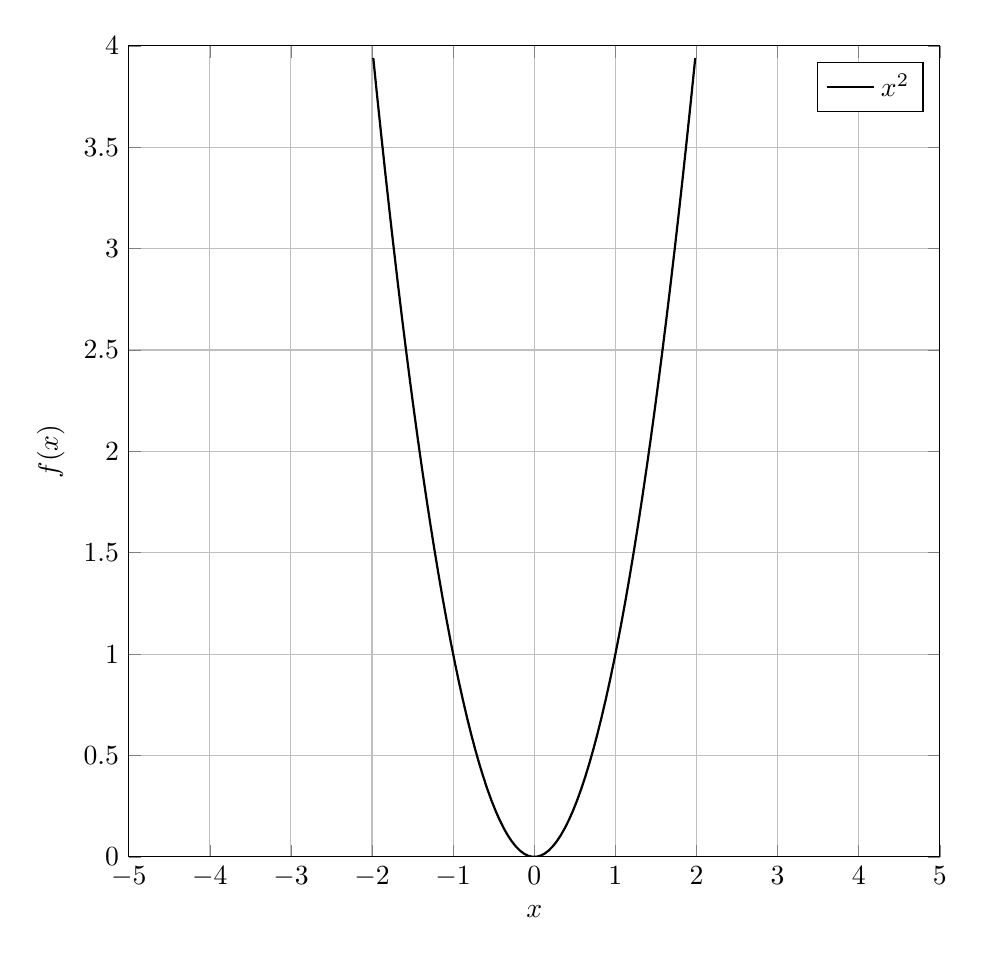
\begin{tikzpicture}
			      \begin{axis}[
					      xmin=-5, xmax=5,
					      ymin=0,ymax=4,
					      restrict y to domain = -4:4, domain=-5:5, width=0.98\textwidth, height=0.98\textwidth, grid=major, samples=200,  ylabel=$f(x)$, xlabel=$x$, legend entries={$ x^2 $}]
				      \addplot[black, thick] {x^2};
			      \end{axis}
		      \end{tikzpicture}
	      \end{minipage}
	      %
	      \begin{minipage}[t]{0.48\textwidth}
		      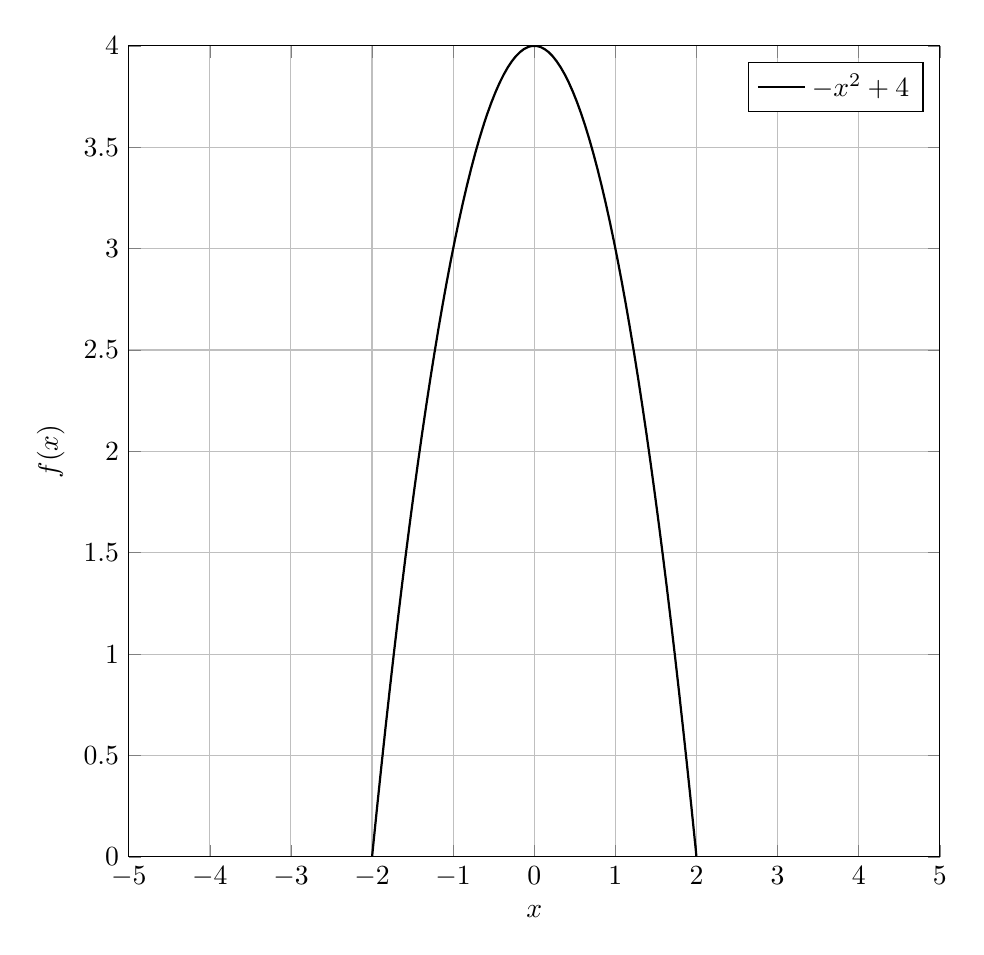
\begin{tikzpicture}
			      \begin{axis}[
					      xmin=-5, xmax=5,
					      ymin=0,ymax=4,
					      restrict y to domain = -4:4, domain=-5:5, width=0.98\textwidth, height=0.98\textwidth, grid=major, samples=200,  ylabel=$f(x)$, xlabel=$x$, legend entries={$ -x^2  + 4$}]
				      \addplot[black, thick] {-x^2 + 4};
			      \end{axis}
		      \end{tikzpicture}
	      \end{minipage}
	\item Il vertice ha coordinate
	      \[
		      \left(\frac{-b}{2a}, \frac{-\Delta }{4a}\right)
	      \]
	\item La parabola incontra l'asse x nelle x che risolvono l'equazione associata (ossia quella ottenuta ponendo la funzione = 0)
	\item Il valore $ c $ è detto \textit{quota}, e indica il punto in cui la parabola incrocia l'asse $ y $
	\item Il coefficiente $ a $, indica quanto "ripida è la parabola"
	      \begin{center}
		      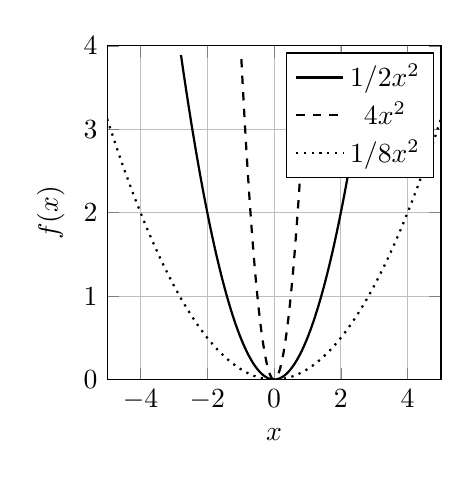
\begin{tikzpicture}
			      \begin{axis}[
					      xmin=-5, xmax=5,
					      ymin=0,ymax=4,
					      restrict y to domain = -4:4, domain=-5:5, width=0.48\textwidth, height=0.48\textwidth, grid=major, samples=200,  ylabel=$f(x)$, xlabel=$x$, legend entries={$ 1/2x^2 $, $4x^2$, $ 1/8 x^2  $}]
				      \addplot[black, thick] {1/2*x^2};
				      \addplot[dashed, thick] {4*x^2};
				      \addplot[dotted, thick] {1/8*x^2};
			      \end{axis}
		      \end{tikzpicture}
	      \end{center}
\end{itemize}

\section{La retta nel piano cartesiano}
Come rappresentiamo una parabola nel piano cartesiano, possiamo rappresentare anche una retta. Se le seguenti sono tutte rette nel piano cartesiano:
\begin{center}
	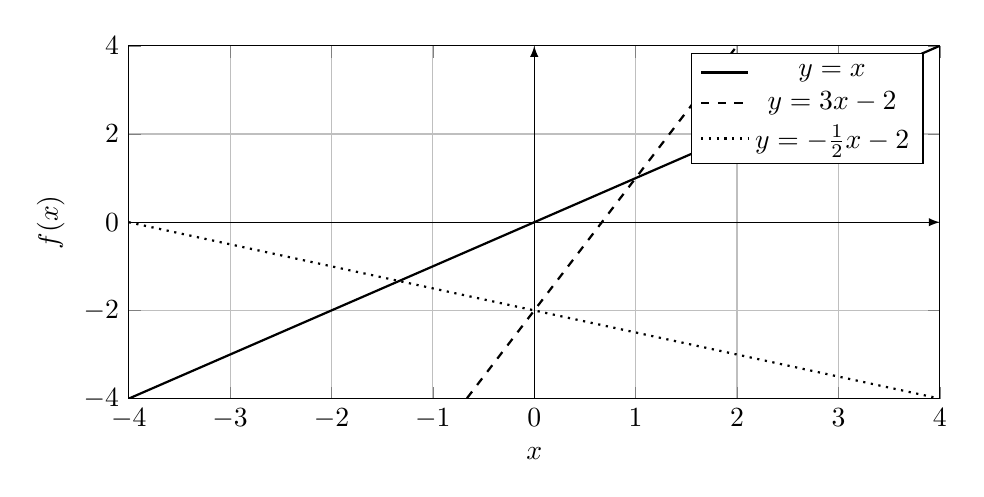
\begin{tikzpicture}
		\begin{axis}[
				xmin=-4, xmax=4,
				ymin=-4,ymax=4,
				restrict y to domain = -4:4, domain=-4:4, width=0.98\textwidth, height=0.5\textwidth, grid=major, samples=200,  ylabel=$f(x)$, xlabel=$x$, legend entries={$y=x$, $ y = 3x -2 $, $ y=-\frac{1}{2} x -2 $}]
			\draw [black, -latex](0,-4)--(0,4);
			\draw [black, -latex](-4,0)--(4,0);
			\addplot[black, thick] {x};
			\addplot[dashed, thick] {3*x -2};
			\addplot[dotted, thick] {-1/2*x -2};
		\end{axis}
	\end{tikzpicture}
\end{center}
Vediamo ora la forma della equazione e cosa considerare per disegnarne una sul piano cartesiano.

\subsection{Equazione retta e grafico}
Una retta ha equazione di tipo:
\[
	y= mx + c
\]
dove $ m $ è detto \textit{coefficiente angolare} e $ c $ è detto, come nelle parabole, \textit{quota}.
\begin{itemize}
	\item $ c $, come nelle parabole, indica l'altezza alla quale la retta interseca l'asse $ y $
	\item $ m $, ossia il coefficiente angolare, indica quanto la retta è inclinata sull'asse orizzontale. Per valori di $ m $ molto grandi, la retta sarà quasi verticale, mentre per valori molto bassi sarà quasi orizzontale. Per valori positivi sarà in "salita" e per valori negativi sarà in "discesa"
\end{itemize}

\subsubsection*{Disegno}
Data una retta con equazione $ y= mx + c $, per ottenere il disegno è sufficiente calcolare due punti e tracciare l'unica retta passante per entrambi. Cinsideriamo
\[
	y = \frac{1}{2}x + 2
\]
\vskip3mm
\begin{minipage}[t]{0.48\textwidth}
	Calcolo $ f\left(-2\right) $ e $ f\left(2\right) $ e segno punti:

	\begin{tikzpicture}
		\begin{axis}[
				xmin=-4, xmax=4,
				ymin=0,ymax=6,
				restrict y to domain = -4:4, domain=-4:4, width=0.98\textwidth, height=0.98\textwidth, grid=major, samples=200,  ylabel=$f(x)$, xlabel=$x$]
			\node (p1)[whitedot, label=90:$p_1$] at (2, {1/2*2 + 2}) {};
			\node (p2)[whitedot, label=90:$p_2$] at (-2, {1/2*-2 + 2}) {};
			\draw [black, -latex](-4, 0)--(4,0);
			\draw [black, -latex](0, 0)--(0, 6);
			\node (o)[] at (0,0) {};
			\draw [dashed] (p2)--(o -| p2);
			\draw [dashed] (p2)--(o |- p2);
			\draw [dashed] (p1)--(o -| p1);
			\draw [dashed] (p1)--(o |- p1);
		\end{axis}
	\end{tikzpicture}
\end{minipage}
%
\begin{minipage}[t]{0.48\textwidth}
	Traccio unica retta passante per entrambi
	\begin{tikzpicture}
		\begin{axis}[
				xmin=-4, xmax=4,
				ymin=0,ymax=6,
				restrict y to domain = -4:4, domain=-4:4, width=0.98\textwidth, height=0.98\textwidth, grid=major, samples=200,  ylabel=$f(x)$, xlabel=$x$, legend entries={$y=\frac{1}{2}x + 2$}]
			\addplot[black, thick] {1/2*x + 2};
			\node (p1)[whitedot, label=90:$p_1$] at (2, {1/2*2 + 2}) {};
			\node (p2)[whitedot, label=90:$p_2$] at (-2, {1/2*-2 + 2}) {};
			\draw [black, -latex](-4, 0)--(4,0);
			\draw [black, -latex](0, 0)--(0, 6);
			\node (o)[] at (0,0) {};
			\draw [dashed] (p2)--(o -| p2);
			\draw [dashed] (p2)--(o |- p2);
			\draw [dashed] (p1)--(o -| p1);
			\draw [dashed] (p1)--(o |- p1);
		\end{axis}
	\end{tikzpicture}
\end{minipage}
\subsubsection*{Ricavare equzione da disegno}
Dato un disegno di una retta, possiamo sfruttare le seguenti proprietà per ricavarne l'equazione come segue:
\begin{itemize}
	\item $ c $ è l'altezza a cui la retta interseca l'asse y
	\item $ m $, dati due punti qualsiasi appartenenti alla retta è uguale a
	      \[
		      m = \frac{y_2 - y_1}{y_2 - y_1} = \frac{\Delta y}{ \Delta x}
	      \]
\end{itemize}
Quindi operativamente, dato un grafico di una retta, per ottenere la sua equazinoe bisogna:
\begin{itemize}
	\item Ricavare il coefficiente angolare, prendendo due punti e dividendo la differenza delle loro $ y $ per la differenza delle loro $ x $
	\item Trovare $ c $ inserendo uno dei due punti della retta e risolvendo un'equazione di primo grado in $ c $
\end{itemize}
\subsubsection*{Esempio}
\begin{tikzpicture}
	\begin{axis}[
			xmin=-2, xmax=6,
			ymin=-2,ymax=4,
			restrict y to domain = -2:6, domain=-2:10, width=0.98\textwidth, height=0.48\textwidth, samples=200,grid = major]
		\addplot[black, thick] {1/2*x + 1};
		\node (p1)[whitedot, label={\contour{white} {$ p_1\left(2,2\right) $} }] at (2, {1/2*2 + 1}) {};
		\node (p2)[whitedot, label={ \contour{white}{$ p_2 \left(4,3\right) $} }] at (4, {1/2*4 + 1}) {};
		\draw [black, -latex](-2,0)--(6,0);
		\draw [black, -latex](0,-2)--(0, 4);
		\node (o)[] at (0,0) {};
		\draw [dashed] (p2)--(o -| p2);
		\draw [dashed] (p2)--(o |- p2);
		\draw [dashed] (p1)--(o -| p1);
		\draw [dashed] (p1)--(o |- p1);
	\end{axis}
\end{tikzpicture}

\begin{enumerate}
	\item Trovare $ m $, ossia il coefficiente angolare:
	      \[
		      m= \frac{\Delta y}{\Delta x} = \frac{y_2-y_1}{x_2 - x_1} = \frac{3 - 2}{4 - 2} = \frac{1}{2}
	      \]
	\item Trovare $ c $, inserendo un punto qualsiasi della retta nella sua equazione:
	      \[
		      y= mx + c \rightarrow y = \frac{1}{2}x + c
	      \]
	      Inserendo $ p_2 $:
	      \[
		      3 = \frac{1}{2} \cdot  4 + c \rightarrow c = 3 - 2 = 1
	      \]
	      oppure inserendo $ p_1 $:
	      \[
		      2 = \frac{1}{2} \cdot  2 + c \rightarrow c = 2 - 1 = 1
	      \]
	\item Quindi, sapendo che $ m=\frac{1}{2} $ e $ c = 1 $, l'equazione della retta sarà:
	      \[
		      y = \frac{1}{2}x + 1
	      \]
	      i
\end{enumerate}


% \textit{Soluzione 1:}
% \begin{align*}
% &4x^2 + 2x - 5 = 0 &  &\underbracket[0.1ex]{(4)}_{a}x^2 + \underbracket[0.1ex]{(2)}_{b}x + \underbracket[0.1ex]{(-5)}_{c} = 0
% \end{align*}
% \begin{center}
%   \begin{tikzpicture}
%   \node (formula)[] at (0,0) {$ \displaystyle x_{1/2} = \frac{-2 \pm \sqrt{2^2 - 4 \cdot 4 \cdot (-5)}}{2 \cdot 4} = \frac{-2 \pm \sqrt{84}}{8} = \frac{-2 \pm 2\sqrt{21}}{8}$}; 
%     \node (solution1)[above right = -0.5em and 2em of formula] {$ \displaystyle x_1 = \frac{-1 + \sqrt{21}}{4} $};
%     \node (solution2)[below right = -0.5em and 2em of formula]  {$ \displaystyle x_2 = \frac{-1 - \sqrt{21}}{4} $};
%     \draw [->] (formula.east) to [out=0, in=180] (solution1.west);
%     \draw [->] (formula.east) to [out=0, in=180] (solution2.west);
%   \end{tikzpicture}
% \end{center}
%
%
% \end{document}
% \begin{align*}
%   &4x^2 + 2x -5 & &\underbracket[0.1ex]{(4)}_{a}x^2 + \underbracket[0.1ex]{(2)}_{b}x + \underbracket[0.1ex]{(-5)}_{c} = 0
% \end{align*}
%   \begin{tikzpicture}
%     \node (formula)[] at (0,0) {$ \displaystyle x_{1/2} = \frac{-2 \pm \sqrt{\left(2\right)^2 -4\left(4\right)\left(-5\right)}}{2 \left(4\right)} = \frac{-2 \pm \sqrt{84}}{28} $}; 
%     \node (solution1)[above right = -0.5em and 2em of formula] {$ \displaystyle x_1 = \frac{12}{4} = 3 $};
%     \node (solution2)[below right = -0.5em and 2em of formula]  {$ \displaystyle x_2 = \frac{-4}{4} = -1 $};
%     \draw [->] (formula.east) to [out=0, in=180] (solution1.west);
%     \draw [->] (formula.east) to [out=0, in=180] (solution2.west);
% \end{tikzpicture} 

\section{Significato di una funzione}
Consideriamo ora una funzione che costituisce una parabola
\[
	x^2  - 4
\]
\begin{center}
	\begin{tikzpicture}
		\begin{axis}[
				xmin=-5, xmax=5,
				ymin=-4,ymax=15,
				restrict y to domain = -40:40, domain=-5:5, width=0.48\textwidth, height=0.48\textwidth, grid=major, samples=200,  ylabel=$f(x)$, xlabel=$x$, legend entries={$x^2 -4 $}]
			\draw [black, thick, -latex](-5,0)--(5,0);
			\draw [black, thick, -latex](0, -4)--(0, 15);
			\addplot[black, thick] {x^2-4};
			\node (h)[whitedot] at (-4, {(-4)^2-4}) {};
			\node (a)[whitedot] at (4, {4^2-4}) {};
			\node (b)[whitedot] at (1, {1^2-4}) {};
			\node (c)[whitedot] at (-1, {(-1)^2-4}) {};
			\node(d)[whitedot] at (2, {2^2-4}) {};
			\node(e)[whitedot] at (-2, {(-2)^2-4}) {};
			\node(f)[whitedot] at (-3, {(-3)^2-4}) {};
			\node(g)[whitedot] at (3, {3^2-4}) {};
			\node (o) at (0,0) {};
			\draw [dashed](a)--(a|-o);
			\draw [dashed](b)--(b|-o);
			\draw [dashed](c)--(c|-o);
			\draw [dashed](d)--(d|-o);
			\draw [dashed](e)--(e|-o);
			\draw [dashed](f)--(f|-o);
			\draw [dashed](g)--(g|-o);
			\draw [dashed](h)--(h|-o);
			%
			\draw [dotted](a)--(a-|o);
			\draw [dotted](b)--(b-|o);
			\draw [dotted](c)--(c-|o);
			\draw [dotted](d)--(d-|o);
			\draw [dotted](e)--(e-|o);
			\draw [dotted](f)--(f-|o);
			\draw [dotted](g)--(g-|o);
			\draw [dotted](h)--(h-|o);
			%
			\node ()[blackdot] at (0,12) {};
			\node ()[blackdot] at (0,5) {};
			\node ()[blackdot] at (0,-3) {};
			%
			\node ()[label=45:{\contour{white}{12}}] at (0,12) {};
			\node ()[label=45:5] at (0,5) {};
			\node ()[label=45:{\contour{white}{-3}}] at (0,-3) {};
		\end{axis}
	\end{tikzpicture}

\end{center}
\begin{center}
	\begin{minipage}[t]{0.48\textwidth}
		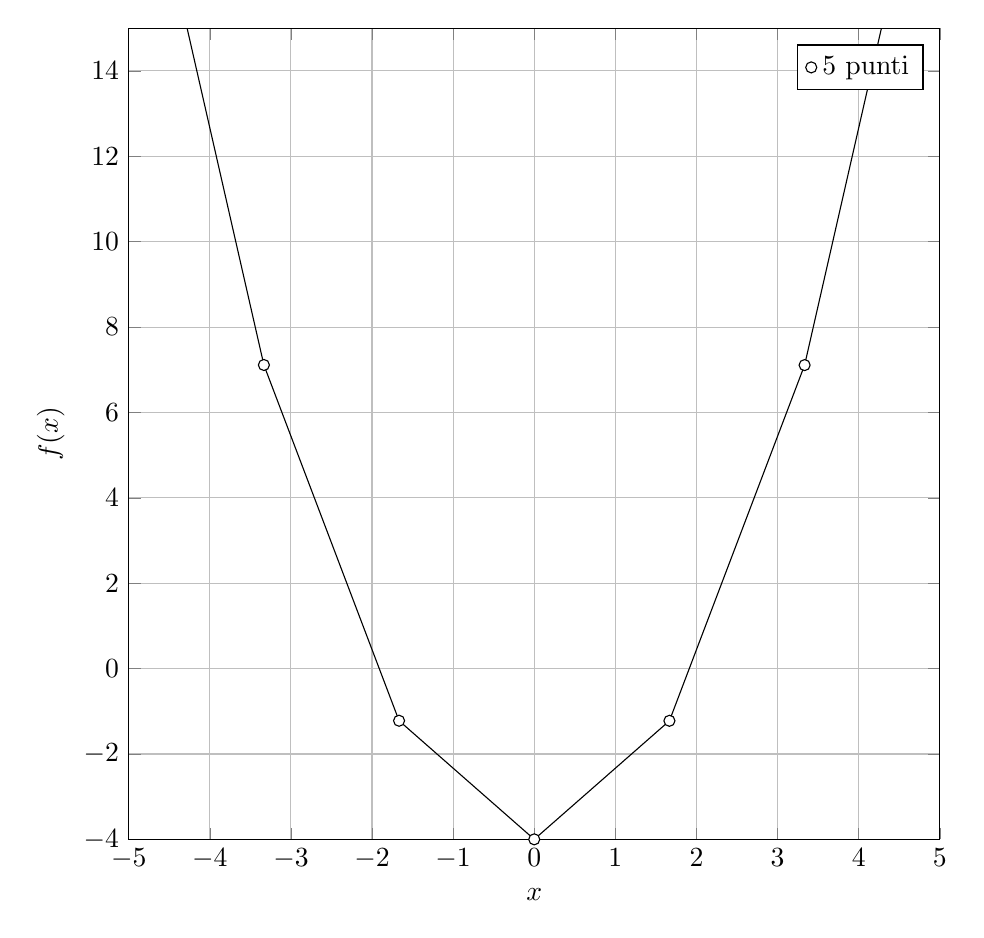
\begin{tikzpicture}
			\begin{axis}[
					xmin=-5, xmax=5,
					ymin=-4,ymax=15,
					restrict y to domain = -40:40, domain=-5:5, width=0.98\textwidth, height=0.98\textwidth, grid=major, samples=7,  ylabel=$f(x)$, xlabel=$x$, legend entries={5 punti}]
				\addplot[only marks, mark=*,
					mark options={               % define custom mark options
							fill=white,                % fill color for the custom mark
							draw=black                % border color for the custom mark
						}, ]
				{x^2-4};
				\addplot[thin] {x^2-4};
			\end{axis}
		\end{tikzpicture}
	\end{minipage}
	%
	\begin{minipage}[t]{0.48\textwidth}
		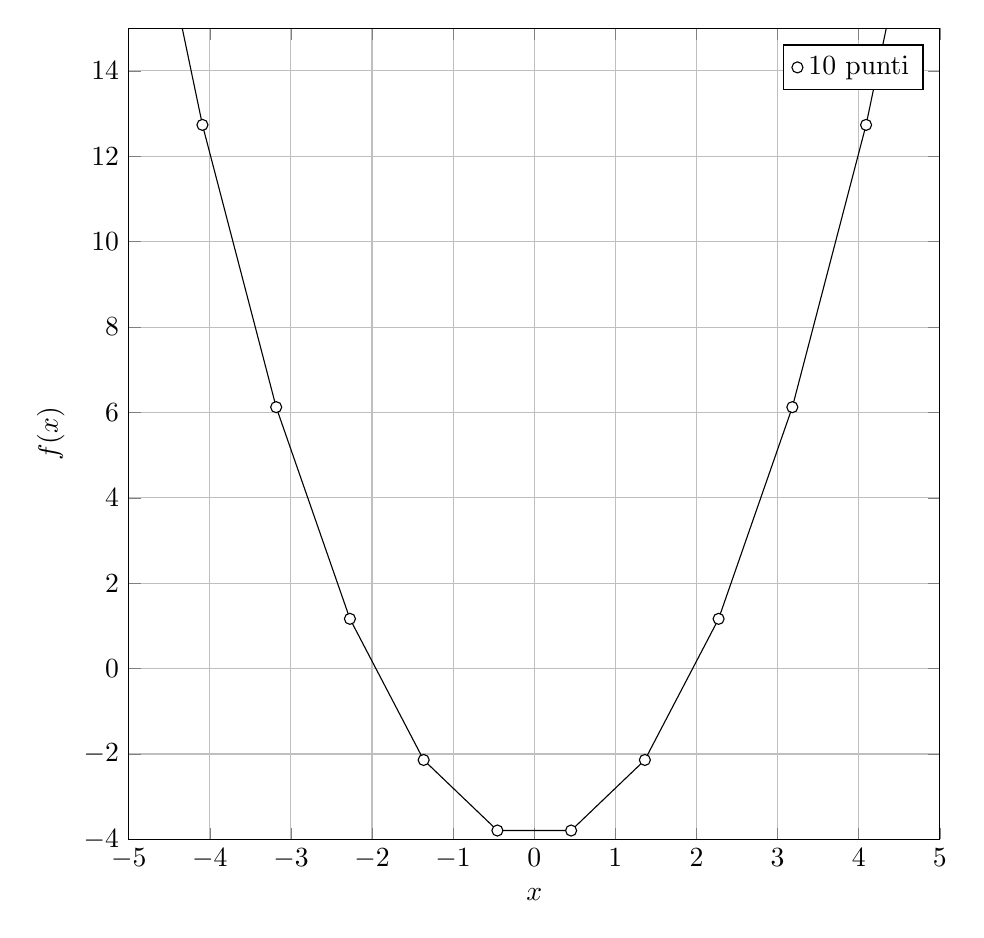
\begin{tikzpicture}
			\begin{axis}[
					xmin=-5, xmax=5,
					ymin=-4,ymax=15,
					restrict y to domain = -40:40, domain=-5:5, width=0.98\textwidth, height=0.98\textwidth, grid=major, samples=12,  ylabel=$f(x)$, xlabel=$x$, legend entries={10 punti}]
				\addplot[only marks, mark=*,
					mark options={               % define custom mark options
							fill=white,                % fill color for the custom mark
							draw=black                % border color for the custom mark
						}, ]
				{x^2-4};

				\addplot[thin] {x^2-4};
			\end{axis}
		\end{tikzpicture}
	\end{minipage}
\end{center}
\begin{center}
	\begin{minipage}[t]{0.48\textwidth}
		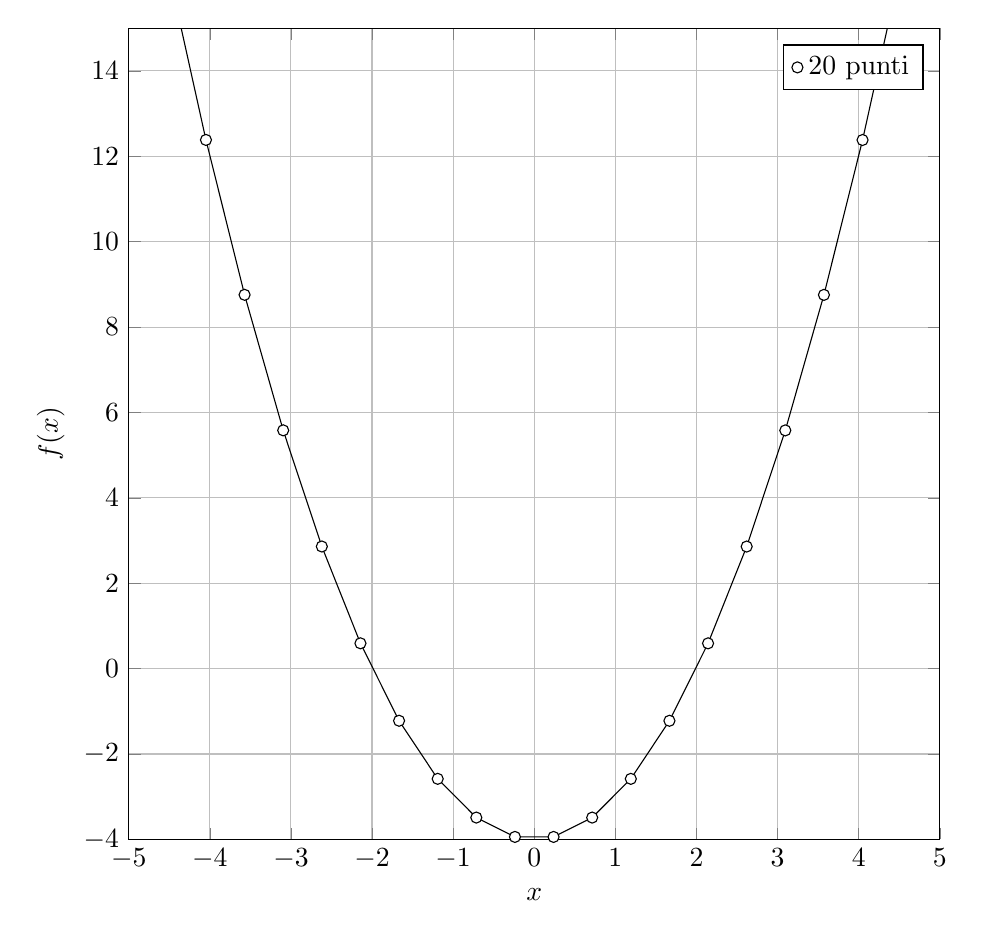
\begin{tikzpicture}
			\begin{axis}[
					xmin=-5, xmax=5,
					ymin=-4,ymax=15,
					restrict y to domain = -40:40, domain=-5:5, width=0.98\textwidth, height=0.98\textwidth, grid=major, samples=22,  ylabel=$f(x)$, xlabel=$x$, legend entries={20 punti}]
				\addplot[only marks, mark=*,
					mark options={               % define custom mark options
							fill=white,                % fill color for the custom mark
							draw=black                % border color for the custom mark
						}, ]
				{x^2-4};
				\addplot[thin] {x^2-4};
			\end{axis}
		\end{tikzpicture}
	\end{minipage}
	%
	\begin{minipage}[t]{0.48\textwidth}
		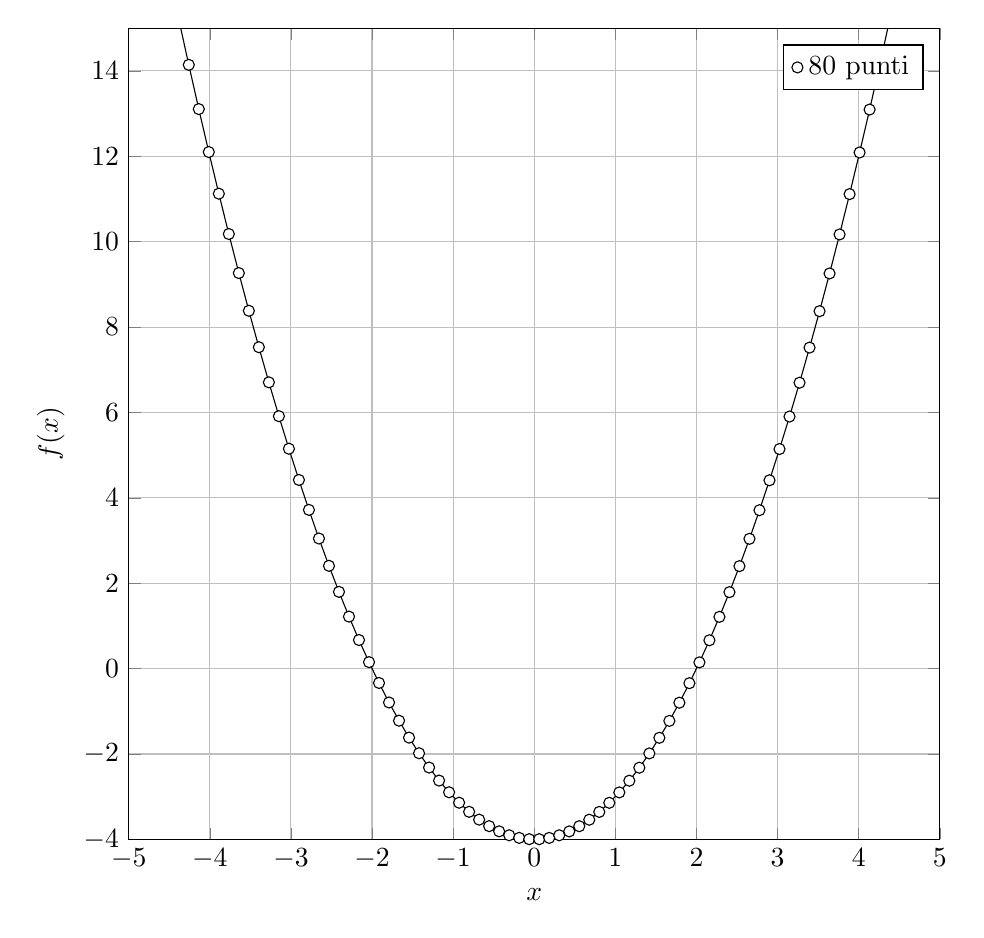
\begin{tikzpicture}
			\begin{axis}[
					xmin=-5, xmax=5,
					ymin=-4,ymax=15,
					restrict y to domain = -40:40, domain=-5:5, width=0.98\textwidth, height=0.98\textwidth, grid=major, samples=82,  ylabel=$f(x)$, xlabel=$x$, legend entries={80 punti}]
				\addplot[only marks, mark=*,
					mark options={               % define custom mark options
							fill=white,                % fill color for the custom mark
							draw=black                % border color for the custom mark
						}, ]
				{x^2-4};
				\addplot[thin] {x^2-4};
			\end{axis}
		\end{tikzpicture}
	\end{minipage}
\end{center}
\section{Sistemi lineari}
\begin{definizione}{Sistema lineare}
	Un sistema lineare è un sistema di equazioni in più incognire dove ogni incognita compare con esponente massimo pari ad 1
\end{definizione}
Ad esempio
\[
	\begin{cases}
		x + 3y - z = 15 \\
		2x -y - z = 0
	\end{cases}
\]
é un sistema lineare, mentre
\[
	\begin{cases}
		x^2  - 2y + 3\sqrt{z} = 12 \\
		2x - xy - z = 0
	\end{cases}
\]
non lo è
\subsection{Soluzioni di un sistema lineare}
Un sistema lineare può avere 0, 1 o infinite soluzioni. Particolare
\begin{itemize}
	\item 1 soluzione se vi sono tante incognite quante equazioni
\end{itemize}

\section{Fisica}
\subsubsection*{Notazione scientifica}
La notazione scientifica è un modo comodo per riscrivere un numero molto grande o molto piccolo. Ad esempio:
\[
	300.000 = 3 \cdot 10 ^{5}
\]
\subsubsection*{Conversione a notazione scientifica}
Per convertire un numero in notazione scientifica occorre seguire questi passaggi:
\begin{enumerate}
	\item Sposta la virgola in maniera tale che resti alla sinistra \textit{solo 1 cifra diversa da 0}, tenendo contro di quanto la abbiamo spostata
	      \[
		      198,274 \text{ diventa } 1,98 \text{ spostando la virgola di } 2 \text{ passi }
	      \]
	\item Moltiplicare il numero ottenuto per $ 10^x $, dove x è quanto abbiamo spostato la virgola e ha segno:
	      \begin{itemize}
		      \item \textit{Positivo} se la abbiamo spostata verso \textit{sinistra}
		      \item \textit{Negativo} se la abbiamo spostata verso \textit{destra}
	      \end{itemize}
	      \[
		      1,98 \cdot 10 ^{2}
	      \]
\end{enumerate}
\subsection{Unità di misura e conversioni}
\begin{center}
	\begin{tabular}{ c c c c c c}
		\toprule
		$ 10^3 $ & $ 10^{2} $ & $ 10^{1} $ & $ 10^{-1} $ & $ 10^{-2} $ & $ 10^{-3} $ \\
		chilo    & etto       & deca       & deci        & centi       & milli       \\
		\bottomrule
	\end{tabular}
	\vskip3mm
	\begin{tabular}{ c c c c c c}
		\toprule
		$ 10^{12} $ & $ 10^{9} $ & $ 10^{6} $ & $ 10^{-6} $ & $ 10^{-9} $ & $ 10^{-12} $ \\
		tera        & mega       & giga       & micro       & nano        & pico         \\
		\bottomrule
	\end{tabular}
\end{center}
\[
	\frac{1}{2} + \int_{a}^{b} f(x) \; dx
\]
\subsection{Moto rettilineo uniformement accelerato}
Nel momento in cui la velocità di un oggetto cambia, si parla di moto rettilineo uniformemente accelerato
Ricordiamo innanzitutto le formule di accelerazione e velocità media:
\begin{minipage}[t]{0.48\textwidth}
	\begin{definizione}{Velocità media}
		La velocità \textit{media}  fra due istanti $ f $ e $ i $ di un corpo è data per definizione dalle seguenti formule:
		\[
			a = \frac{\Delta v}{\Delta t} = \frac{v_f - v_i}{t_f - t_i}
		\]
	\end{definizione}

\end{minipage}
\hfill
%
\begin{minipage}[t]{0.48\textwidth}
	\begin{definizione}{Velocità media}
		L'accelerazione  fra due istanti $ f $ e $ i $ di un corpo è data per definizione dalle seguenti formule:
		\[
			v_m = \frac{\Delta s}{\Delta t} =  \frac{x_f - x_i}{t_f - t_i}
		\]
	\end{definizione}

\end{minipage}
\begin{definizione}{Accelerazione e velocità media}
	La velocità \textit{media} e accelerazione fra due istanti $ f $ e $ i $ di un corpo è data per definizione dalle seguenti formule:
	\begin{align*}
		 & a = \frac{\Delta v}{\Delta t} = \frac{v_f - v_i}{t_f - t_i} &  & v_m = \frac{\Delta s}{\Delta t} =  \frac{x_f - x_i}{t_f - t_i}
	\end{align*}

\end{definizione}

Inoltre, la formula più importante di tutte da tenere a mente è la legge oraria:
\begin{definizione}{Legge oraria MRUA}
	Dato un corpo che si muove di moto rettilineo uniformemente accelerato, la sua posizione in funzione del tempo è data da
	\[
		x = \frac{1}{2} a t^2 + vt + x_0
	\]
\end{definizione}
L'ultima formula che serve sapere è quella che collega la velocità all'accelerazione:
\begin{definizione}{Rapporto tra velocità e accelerazione}
	Dato un corpo con accelerazione costante $ a $ e velocità iniziale $ v_0 $, la sua velocità dopo $ t $ secondi è data da:
	\[
		v = + at + v_0
	\]
\end{definizione}
\end{document}
